\documentclass[aspectratio=169,11pt]{beamer}

% ============================================================
% PACKAGES
% ============================================================
\usepackage{graphicx}
\usepackage{tikz}
\usetikzlibrary{positioning,arrows.meta,calc}
\usepackage{xcolor}
\usepackage{booktabs}
\usepackage{tabularx}
\usepackage{array}
\usepackage{ragged2e}
\usepackage{hyperref}

% ============================================================
% COLORS - SAME AS PHASE-I
% ============================================================
\definecolor{GEUBlue}{RGB}{20,55,105}
\definecolor{GEULightBlue}{RGB}{238,244,251}
\definecolor{GEUGrey}{RGB}{90,90,90}
\definecolor{GEULightGrey}{RGB}{245,246,248}

% ============================================================
% BEAMER SETTINGS
% ============================================================
\usetheme{default}
\setbeamertemplate{navigation symbols}{}
\setbeamertemplate{blocks}[rounded][shadow=false]

\setbeamercolor{normal text}{fg=black,bg=white}
\setbeamercolor{frametitle}{fg=GEUBlue}
\setbeamercolor{structure}{fg=GEUBlue}
\setbeamercolor{block title}{fg=GEUBlue,bg=GEULightBlue}
\setbeamercolor{block body}{fg=black,bg=GEULightBlue}

\setbeamerfont{frametitle}{size=\Large,series=\bfseries}

% ============================================================
% LOGO
% ============================================================
% Upload the Graphic Era logo with this filename to Overleaf.
\newcommand{\GEULogo}{graphicera_logo.png}
% The logo is optional: compilation still works if the image is not uploaded.
\newcommand{\SafeLogo}{%
  \IfFileExists{\GEULogo}{\includegraphics[height=0.62cm]{\GEULogo}}{}%
}

% ============================================================
% HEADER
% ============================================================
\setbeamertemplate{headline}{%
  \begin{tikzpicture}[remember picture,overlay]
    \node[
        anchor=north east,
        xshift=-0.30cm,
        yshift=-0.12cm
    ] at (current page.north east)
    {\SafeLogo};
  \end{tikzpicture}
  \vspace{0.72cm}
}

% ============================================================
% FRAME TITLE
% ============================================================
\setbeamertemplate{frametitle}{%
  \vspace{0.03cm}
  \insertframetitle\par
  \vspace{0.04cm}
  \textcolor{GEUBlue}{\rule{\textwidth}{0.9pt}}
  \vspace{0.03cm}
}

% ============================================================
% FOOTER
% ============================================================
\setbeamertemplate{footline}{%
  \leavevmode
  \hbox{%
  \begin{beamercolorbox}[
      wd=.82\paperwidth,
      ht=0.32cm,
      dp=0.10cm,
      leftskip=.3cm
  ]{author in head/foot}
    \tiny Department of Computer Science \& Engineering |
    Graphic Era (Deemed to be University)
  \end{beamercolorbox}%
  \begin{beamercolorbox}[
      wd=.18\paperwidth,
      ht=0.32cm,
      dp=0.10cm,
      rightskip=.3cm
  ]{date in head/foot}
    \hfill\tiny\insertframenumber/\inserttotalframenumber
  \end{beamercolorbox}}
}

% ============================================================
% CUSTOM COMMANDS
% ============================================================
\newcommand{\smallnote}[1]{%
\vspace{0.08cm}
{\scriptsize\color{GEUGrey}#1}
}

\newcommand{\placeholder}[1]{%
\textit{\color{GEUGrey}#1}
}

% ============================================================
% DOCUMENT INFORMATION
% ============================================================
\title{\textbf{Project-Based Learning}\\[2mm]\large Phase-II Evaluation}
\author{\textbf{FOOD RESCUE}\\Smart Food Rescue and Redistribution System\\Team ID: DSCPP-III-2026-T381}

\institute{
Department of Computer Science \& Engineering\\
Graphic Era (Deemed to be University), Dehradun
}

\date{Academic Session 2026--27}

% ============================================================
% DOCUMENT
% ============================================================
\begin{document}

% ============================================================
% SLIDE 1
% ============================================================
\begin{frame}[plain]

\begin{tikzpicture}[remember picture,overlay]

\draw[GEUBlue,line width=3pt]
(current page.north west) -- (current page.north east);

\node[
    anchor=north east,
    xshift=-0.45cm,
    yshift=-0.35cm
] at (current page.north east)
{\IfFileExists{\GEULogo}{\includegraphics[height=1.0cm]{\GEULogo}}{}};

\node[
    align=center,
    text width=.84\paperwidth
] at ([yshift=.25cm]current page.center)
{
{\color{GEUBlue}
\fontsize{26}{30}\selectfont
\bfseries PROJECT-BASED LEARNING}
\\[3mm]

{\fontsize{18}{22}\selectfont
PHASE-II EVALUATION}
\\[7mm]

{\color{GEUGrey}
\Large\bfseries
\textbf{FOOD RESCUE}\\[1mm]\large Smart Food Rescue and Redistribution System}
\\[3mm]

{\color{GEUBlue}
\normalsize Team ID: DSCPP-III-2026-T381}
};

\node[
    align=center,
    anchor=south,
    yshift=.42cm
] at (current page.south)
{
\bfseries
Department of Computer Science \& Engineering\\
Graphic Era (Deemed to be University), Dehradun\\[-1mm]
\scriptsize Academic Session 2026--27
};

\end{tikzpicture}

\end{frame}

% ============================================================
% SLIDE 2
% ============================================================
\begin{frame}{Team \& Mentor Details}

\begin{columns}[T,totalwidth=\textwidth]

\column{.48\textwidth}

\begin{block}{Team Information}
\begin{tabular}{@{}ll@{}}
\textbf{Team ID:} & DSCPP-III-2026-T381\\
\textbf{Semester:} & 3rd\\
\textbf{Section:} & ML2, ML3, DS1, ML4\\
\textbf{Domain:} & Social Impact
\end{tabular}
\end{block}

\column{.48\textwidth}

\begin{block}{Team Members}
1.\quad Aditya Dutta (Lead) -- 2510373905\\
2.\quad Utsav Bajoria -- 2510370581\\
3.\quad Vishwajeet Singh -- 2510380298\\
4.\quad Raghav Pandey -- 2510380113
\end{block}

\end{columns}

\vspace{2mm}

\begin{block}{Mentor}
Mr. Chirag Tyagi
\hfill
\textbf{Interactions completed:}
\underline 8 {\hspace{12mm}}
\end{block}

\vfill

\smallnote{
Brief Discussion: Introduce the team, project domain, mentor,
and responsibilities of the team members.
}

\end{frame}

% ============================================================
% SLIDE 3
% ============================================================
\begin{frame}{Phase-I Recap \& Feedback Incorporated}

\begin{block}{Phase-I Status}
Literature/background study on food-rescue platforms completed; requirements and user roles finalized; system architecture and class diagram prepared.
\end{block}

\vspace{2mm}

\begin{columns}[T,totalwidth=\textwidth]

\column{.48\textwidth}

\textbf{\color{GEUBlue}Feedback Received}

\begin{itemize}\itemsep2pt
\item Improve donation prioritization.
\item Improve coordination between NGOs and donors.
\item Make delivery planning more efficient.
\end{itemize}

\column{.48\textwidth}

\textbf{\color{GEUBlue}Changes Incorporated}

\begin{itemize}\itemsep2pt
\item Design priority selection based on expiry and urgency.
\item Plan requirement-based donation matching.
\item Include distance-based route planning.
\end{itemize}

\end{columns}

\vfill

\smallnote{
Brief Discussion: Explain the major feedback received during Phase-I
and clearly demonstrate how it has been incorporated.
}

\end{frame}

% ============================================================
% SLIDE 4
% ============================================================
\begin{frame}{Problem Statement \& Finalized Objectives}

\begin{block}{Problem Statement}
Restaurants, hostels, households, and events often generate surplus food that is still safe to consume, while NGOs and people in need may face shortages. Without proper coordination, usable food goes to waste. Food Rescue connects donors with NGOs and records food quantity, location, type, and expiry, prioritizing donations by urgency and distance.
\end{block}

\vspace{2mm}

\textbf{\color{GEUBlue}Finalized Objectives}

\begin{enumerate}\itemsep3pt
\item Reduce food wastage by connecting food donors with NGOs and volunteers.
\item Match surplus food with NGO requirements by food type, quantity, and location.
\item Prioritize eligible donations based on expiry time and urgency.
\item Support efficient pickup and delivery route planning using graph algorithms.
\end{enumerate}

\vfill

\smallnote{
Brief Discussion: Avoid repeating the complete Phase-I presentation.
Focus on the finalized problem, scope and measurable objectives.
}

\end{frame}

% ============================================================
% SLIDE 5
% ============================================================
\begin{frame}{Updated System Architecture / Workflow}

\begin{center}

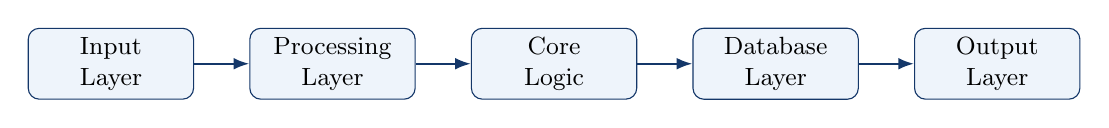
\begin{tikzpicture}[
node distance=7mm,
box/.style={
rectangle,
rounded corners,
draw=GEUBlue,
fill=GEULightBlue,
minimum width=2.10cm,
minimum height=9mm,
align=center,
font=\small
},
arrow/.style={
-{Latex[length=2mm]},
thick,
draw=GEUBlue
}
]

\node[box] (a) {Input\\Layer};
\node[box,right=of a] (b) {Processing\\Layer};
\node[box,right=of b] (c) {Core\\Logic};
\node[box,right=of c] (d) {Database\\Layer};
\node[box,right=of d] (e) {Output\\Layer};

\draw[arrow] (a)--(b);
\draw[arrow] (b)--(c);
\draw[arrow] (c)--(d);
\draw[arrow] (d)--(e);

\end{tikzpicture}

\end{center}

\vspace{4mm}

\begin{columns}[T,totalwidth=\textwidth]

\column{.48\textwidth}

\textbf{\color{GEUBlue}Major Components}

\begin{itemize}\itemsep2pt
\item UI layer for donors, NGOs, and volunteers.
\item Logic engine for constraint checking and donation allocation.
\item Record management for donations, users, and deliveries.
\end{itemize}

\column{.48\textwidth}

\textbf{\color{GEUBlue}Changes Since Phase-I}

\begin{itemize}\itemsep2pt
\item Defined a modular, layered architecture.
\item Added priority-based matching and route-planning logic.
\item Connected donor, NGO, and volunteer workflows.
\end{itemize}

\end{columns}

\vfill

\smallnote{
Brief Discussion: Present the updated architecture and explain
how individual modules communicate with each other.
}

\end{frame}

% ============================================================
% SLIDE 6
% ============================================================
\begin{frame}{Module Design \& Functional Requirements}
\small
\begin{columns}[T,totalwidth=\textwidth]
\column{.48\textwidth}
\textbf{\color{GEUBlue}Major Modules}
\begin{enumerate}\itemsep1pt\parskip0pt
\item Core DSA, Integration \& UI
\item Volunteer \& Delivery Module
\item NGO \& Requirement Module
\item Donor \& Food Donation Module
\end{enumerate}
\column{.48\textwidth}
\textbf{\color{GEUBlue}Functional Requirements}
\begin{itemize}\itemsep1pt\parskip0pt
\item Web front-end (HTML/CSS/JavaScript) for three user roles.
\item Priority-based donation selection and matching.
\item Dijkstra-based delivery route planning.
\item Delivery tracking and file-based record storage.
\end{itemize}
\end{columns}
\vspace{-2mm}
\begin{block}{Module Dependency / Data Flow}
\centering

\begin{tikzpicture}[
  node distance=2.5mm,
  flowbox/.style={rectangle,rounded corners=2pt,draw=GEUBlue,fill=GEULightBlue,
    text width=2.55cm,minimum height=0.72cm,align=center,font=\tiny,inner sep=2pt},
  coreflow/.style={rectangle,rounded corners=2pt,draw=GEUBlue,fill=GEUBlue,
    text=white,text width=2.55cm,minimum height=0.72cm,align=center,font=\tiny\bfseries,inner sep=2pt},
  flowarrow/.style={-{Latex[length=1.5mm]},thick,draw=GEUBlue}
]
\node[flowbox] (donor) {Donor \& Food Donation\\Records surplus food};
\node[flowbox,right=of donor] (ngo) {NGO \& Requirement\\Provides food needs};
\node[coreflow,right=of ngo] (core) {Core DSA / Matching\\Selects suitable donations};
\node[flowbox,right=of core] (vol) {Volunteer \& Delivery\\Pickup and status};
\draw[flowarrow] (donor) -- (ngo);
\draw[flowarrow] (ngo) -- (core);
\draw[flowarrow] (core) -- (vol);
\end{tikzpicture}
\end{block}
\end{frame}

% ============================================================
% SLIDE 7
% ============================================================
\begin{frame}{Technology Stack \& Development Methodology}

\begin{columns}[T,totalwidth=\textwidth]

\column{.48\textwidth}

\begin{block}{Technology Stack}

\begin{itemize}\itemsep2pt
\item Programming: C++ (STL, OOP, DSA), HTML, CSS, JavaScript
\item Data storage: File-based CSV / text records
\item Library: Standard Template Library (STL)
\item Development tool: VS Code / Code::Blocks
\item Version control: Git / GitHub
\end{itemize}

\end{block}

\column{.48\textwidth}

\begin{block}{Development Methodology}

\begin{enumerate}\itemsep2pt
\item Requirement Analysis
\item System Design
\item Module Development
\item Integration
\item Testing \& Validation
\end{enumerate}

\end{block}

\end{columns}

\vfill

\smallnote{
Brief Discussion: Explain why the selected technologies are appropriate
and how the team is following the development methodology.
}

\end{frame}

% ============================================================
% SLIDE 8
% ============================================================
\begin{frame}{Implementation of PBL Course Concepts}

\scriptsize
\renewcommand{\arraystretch}{1.3}
\setlength{\tabcolsep}{5pt}

\begin{tabularx}{\textwidth}
{@{}>{\raggedright\arraybackslash\bfseries}p{2.25cm}
>{\raggedright\arraybackslash}X
>{\raggedright\arraybackslash}p{2.35cm}@{}}
\toprule
Course & Concepts Actually Implemented & Project Module\\
\midrule
Data Structures in C &
Priority queue for urgent donations; queue for NGO requests; hash table for donor/NGO/volunteer lookup; graph and Dijkstra's algorithm for delivery routes. &
DSA-based matching and optimization\\
\addlinespace[3pt]
OOPs with C++ &
Classes for Donor, FoodDonation, NGO, Volunteer, Requirement, and Delivery; STL containers and file handling. Include inheritance/polymorphism only if implemented. &
Application and data-management layer\\
\bottomrule
\end{tabularx}

\vfill
\begin{center}
\colorbox{GEULightBlue}{
\parbox{.92\textwidth}{
\centering
\textbf{Important:} Mention only concepts actually implemented in the project.
}}
\end{center}

\smallnote{Be prepared to explain where and how each concept is used in the code.}

\end{frame}

% ============================================================
% SLIDE 9
% ============================================================
\begin{frame}{Development \& Implementation Progress}

\scriptsize

\begin{center}

\renewcommand{\arraystretch}{1.25}

\begin{tabularx}{.96\textwidth}
{@{}p{3cm}p{2.2cm}X@{}}

\toprule
\textbf{Module} &
\textbf{Status} &
\textbf{Work Completed}\\
\midrule

Core DSA, Integration \& UI &
in-progress &
Implement core data structures and coordinate module integration.\\

Volunteer \& Delivery &
Completed &
Implement core data structures and coordinate module integration.\\

NGO \& Requirement &
Completed&
Develop NGO requirement matching and validate matching cases.\\

Donor \& Food Donation &
Completed &
Complete donor records, integration, testing, and documentation as needed.\\

\bottomrule

\end{tabularx}

\end{center}

\vspace{3mm}

\begin{center}
\colorbox{GEULightBlue}{
\parbox{.65\textwidth}{
\centering
\textbf{Overall Project Completion:}
\placeholder{Enter actual percentage based on completed work}
}}
\end{center}

\vfill

\smallnote{
Brief Discussion: Clearly differentiate between completed,
in-progress and pending development. Do not present proposed work
as completed work.
}

\end{frame}

% ============================================================
% SLIDE 10
% ============================================================
\begin{frame}{Working Prototype / Demonstration}

\begin{columns}[T,totalwidth=\textwidth]

\column{.45\textwidth}

\textbf{\color{GEUBlue}Implemented Features}

\begin{itemize}\itemsep3pt
\item Food donation entry and record management (if working).
\item NGO requirement registration and matching (if working).
\item Priority-based donation selection (if working).
\item Volunteer assignment / route planning (if working).
\end{itemize}

\column{.51\textwidth}

\begin{block}{Prototype / Output}

\centering
\vspace{1mm}
\includegraphics[height=5.0cm,width=\linewidth,keepaspectratio]{food_rescue_screenshot.png}
\vspace{1mm}

\end{block}

\end{columns}

\vfill

\smallnote{
Brief Discussion: Demonstrate the actual working implementation.
Students should preferably provide a live demonstration in addition
to screenshots wherever applicable.
}

\end{frame}

% ============================================================
% SLIDE 11
% ============================================================
\begin{frame}{Testing, Results \& Validation}
\scriptsize
\renewcommand{\arraystretch}{1.0}
\setlength{\tabcolsep}{3pt}
\begin{center}
\begin{tabularx}{.97\textwidth}{@{}p{1.55cm}X X p{1.15cm}@{}}
\toprule
\textbf{Test / Module} & \textbf{Expected Result} & \textbf{Evidence in Test Code} & \textbf{Status}\\
\midrule
Donor / volunteer & Registered records display. & Calls to \texttt{displayDonor()} and \texttt{displayAll()}. & Code present\\
NGO matching & Rice donation (20 units) checked against 20-unit requirement. & Calls to \texttt{matchWithDonations()} and pending/fulfilled displays. & Verify output\\
Priority queue & One queued task is processed. & Three tasks enqueued; \texttt{dequeue()} processes one. & Verify output\\
Volunteer assignment & Volunteer assigned to intended delivery. & Creates delivery ID 401 but searches for ID 501. & Fix ID mismatch\\
\bottomrule
\end{tabularx}
\end{center}
\vspace{2mm}
\begin{beamercolorbox}[rounded=true,sep=4pt,wd=.97\textwidth]{block body}
\textbf{Results / Validation:} Run tests and record console output before marking Pass. Fix ID mismatch: delivery 401 is created, but 501 is searched.
\end{beamercolorbox}
\end{frame}

% SLIDE 12
% ============================================================
\begin{frame}{GitHub Repository \& Development Activity}

\begin{columns}[T,totalwidth=\textwidth]

\column{.46\textwidth}

\textbf{\color{GEUBlue}Repository Information}

\begin{itemize}\itemsep3pt
\item GitHub Link: \href{https://github.com/}{Insert actual repository URL}
\item README.md: Updated
\item Contributors: Aditya Dutta , Utsav Bajoria , 
                    Vishwajeet Singh , Raghav Pandey
\item Repository Status: Updated
\item Branches: Main
\end{itemize}

\column{.50\textwidth}

\textbf{\color{GEUBlue}Development Activity}

\begin{itemize}\itemsep3pt
\item Commit history maintained by each member.
\item Use descriptive commit messages.
\item Individual work visible in commit history.
\item Upload latest tested implementation.
\item Maintain README and setup instructions.
\end{itemize}

\end{columns}

\vfill

\begin{center}
\colorbox{GEULightBlue}{
\parbox{.88\textwidth}{
\centering
\textbf{Requirement:}
All team members must be contributors and must
\textbf{commit individually using their own GitHub accounts}.
}}
\end{center}

\smallnote{
Brief Discussion: Show repository activity, README, contributor list
and commit history during the presentation.
}

\end{frame}

% ============================================================
% SLIDE 13
% ============================================================
\begin{frame}{Individual Contribution}

\scriptsize

\begin{center}

\renewcommand{\arraystretch}{1.35}

\begin{tabularx}{.96\textwidth}
{@{}p{2.0cm}p{2.0cm}X p{1.6cm}@{}}

\toprule
Member &
Role &
Technical Contribution &
GitHub Commits\\
\midrule

Aditya Dutta &
Core DSA, Integration \& UI &
Core data structures, integration, and UI work actually completed. &
27\\

Utsav Bajoria &
Volunteer \& Delivery &
Volunteer records, pickup assignment, and delivery tracking, where implemented. &
7\\

Vishwajeet Singh &
NGO \& Requirement &
NGO requirement records and donation-matching work, where implemented. &
9\\

Raghav Pandey &
Donor \& Food Donation &
Donor records and food donation entry, where implemented. &
7\\

\bottomrule

\end{tabularx}

\end{center}

\vspace{3mm}

\begin{block}{Individual Evaluation}
Every member should be prepared to explain and demonstrate
their own technical contribution to the project.
\end{block}

\smallnote{
Brief Discussion: Contributions should be specific and verifiable.
Avoid generic statements such as ``helped in coding'' or
``worked on documentation''.
}

\end{frame}

% ============================================================
% SLIDE 14
% ============================================================
\begin{frame}{Challenges, Remaining Work \& Phase-III Roadmap}
\small
\begin{columns}[T,totalwidth=\textwidth]
\column{.48\textwidth}
\textbf{\color{GEUBlue}Challenges Faced}
\begin{itemize}\itemsep1pt\parskip0pt\topsep2pt
\item Ensuring suitable donation-to-NGO matching.
\item Coordinating interfaces and records across modules.
\item Maintaining correct priority and delivery records.
\end{itemize}
\vspace{1mm}
\textbf{\color{GEUBlue}Solutions / Learning}
\begin{itemize}\itemsep1pt\parskip0pt\topsep2pt
\item Use modular design, suitable data structures, and test cases.
\item Apply DSA and OOP concepts to a practical social-impact problem.
\end{itemize}
\column{.48\textwidth}
\textbf{\color{GEUBlue}Phase-III Roadmap}
\begin{enumerate}\itemsep2pt\parskip0pt\topsep2pt
\item Complete remaining module implementations.
\item Integrate donor, NGO, volunteer, and core logic.
\item Test edge cases and optimize matching and routes.
\item Demonstrate and validate the final prototype.
\item Complete README, test evidence, and final report.
\end{enumerate}
\end{columns}
\end{frame}

% ============================================================
% SLIDE 15
% ============================================================
\begin{frame}{Expected Outcomes \& References}

\begin{columns}[T,totalwidth=\textwidth]

\column{.47\textwidth}

\textbf{\color{GEUBlue}Expected Final Outcomes}

\begin{itemize}\itemsep3pt
\item Integrated working food-rescue prototype.
\item Validated donation matching and route-planning results.
\item Potential use by donors, NGOs, and volunteers.
\item Future extension to live maps and persistent databases.
\item Potential for further evaluation and improvement.
\end{itemize}

\column{.47\textwidth}

\textbf{\color{GEUBlue}References}

\begin{enumerate}\itemsep3pt
\item Cormen et al., Introduction to Algorithms.
\item Balagurusamy, Object-Oriented Programming with C++.
\item C++ Standard Library documentation.
\item Course lecture notes on Data Structures and OOP.
\item Add the actual project GitHub repository URL.
\end{enumerate}

\vfill

\begin{center}

\colorbox{GEUBlue}{
\parbox{.78\textwidth}{
\centering
\color{white}
\textbf{Thank You}\\
Questions \& Suggestions
}}

\end{center}

\end{columns}

\vfill

\smallnote{
Brief Discussion: Conclude with the tangible final outcome expected
from the project and cite the major technical/research resources used.
}

\end{frame}

\end{document}
